\documentclass{article}
\usepackage[a4paper, portrait, margin=1.5cm]{geometry}
\usepackage[utf8]{inputenc}
\usepackage[english]{babel}
\usepackage{longtable}
\usepackage{graphicx}
\graphicspath{ {images/} }
\usepackage{biblatex}
\addbibresource{resources.bib}
\usepackage{hyperref}
\usepackage{listings}

\title{Data Exploration of NYC Subway Dataset}
\author{Ivailo Kassamakov}
\date{October 2015}
\begin{document}

\maketitle
\begin{abstract}
The present project is an effort towards fulfilling the requirements of the Data Analyst Nanodegree at Udacity.

The goal is to perform exploratory data analysis on a dataset collected from readings of weather sensors and turnstile counters situated at the stations of the NYC subway.

All calculations and graphics have been done within an IPython notebook (an indispensable part of this project), with the \tt pandas\rm, \tt statmodels \rm and \tt matplotlib \rm packages.

Ideas, explanations and guidelines for using Pandas and (I)Python have been taken from \cite{anthony2015mastering}, \cite{mckinney2013python}, and \cite{rossant2013learning}.

Some useful tools used during the work on this project were: \href{www.sharelatex.com}{www.sharelatex.com}, \href{www.tablesgenerator.com}{www.tablesgenerator.com}, \href{www.ottobib.com}{www.ottobib.com}, and \href{www.maptiler.org}{www.maptiler.org}.
\end{abstract}

\tableofcontents

\listoffigures
 
\listoftables

\section{Introduction}

The input dataset comes as a CSV file containing 42649 records. Each record consist of 27 columns, and their meaning is given in table \ref{tab:col_meaning}.

\begin{longtable}[h]{c|l|p{8cm}}

\hline
No. & Column name & Column Description \\[3pt]
\hline
\endfirsthead

%\hline
\multicolumn{3}{c}{(Table Cont'd)}\\
\hline
No. & Column name & Column Description \\[3pt]
\hline

\endhead

\hline
\multicolumn{3}{c}{(Continues on next page)}\\
\endfoot


\hline
\caption{Meaning of the columns in the input dataset
\label{tab:col_meaning}}
\endlastfoot

 1 & UNIT & Remote unit that collects turnstile information. Can collect from multiple banks of turnstiles. Large subway stations can have more than one unit. \\[3pt]
 
2 & DATEn & Date in “yyyy-mm-dd” (2011-05-21) format. \\[3pt]

3 & TIMEn & Time in “hh:mm:ss” (08:05:02) format. \\[3pt]

4 & ENTRIESn & Raw reading of cumulative turnstile entries from the remote unit. Occasionally resets to 0. \\[3pt]

5 & EXITSn & Raw reading of cumulative turnstile exits from the remote unit. Occasionally resets to 0. \\[3pt]

6 & ENTRIESn\_hourly & Difference in ENTRIES from the previous REGULAR reading.\\[3pt] 

7 & EXITSn\_hourly & Difference in EXITS from the previous REGULAR reading. \\[3pt]

8 & datetime & Date and time in “yyyy-mm-dd hh:mm:ss” format (2011-05-01 00:00:00). Can be parsed into a Pandas \tt datetime \rm object without modifications. \\[3pt]

9 & hour & Hour of the timestamp from TIMEn. Truncated rather than rounded. \\[3pt]

10 & day\_week & Integer (0--6 Mon--Sun) corresponding to the day of the week. \\[3pt]

11 & weekday & Indicator (0 or 1) if the date is a weekday (Mon--Fri). \\[3pt]

12 & station & Subway station corresponding to the remote unit. \\[3pt]

13 & latitude & Latitude of the subway station corresponding to the remote unit.  \\[3pt]

14 & longitude & Longitude of the subway station corresponding to the remote unit. \\[3pt]

15 & conds & Categorical variable of the weather conditions (Clear, Cloudy etc.) for the time and location. \\[3pt]

16 & fog & Indicator (0 or 1) if there was fog at the time and location. \\[3pt]

17 & precipi & Precipitation in inches at the time and location. \\[3pt]

18 & pressurei & Barometric pressure in inches Hg at the time and location. \\[3pt] 

19 & rain  & Indicator (0 or 1) if rain occurred within the calendar day at the location. \\[3pt]

20 & tempi & Temperature in $^{\circ}{\rm F}$ at the time and location. \\[3pt]

21 & wspdi & Wind speed  in mph at the time and location. \\[3pt]

22 & meanprecipi & Daily average of \tt precipi \rm for the location. \\[3pt]

23 & meanpressurei & Daily average of \tt pressurei \rm for the location. \\[3pt]

24 & meantempi & Daily average of \tt tempi \rm for the location. \\[3pt]

25 & meanwspdi & Daily average of \tt wspdi \rm for the location. \\[3pt]

26 & weather\_lat & Latitude of the weather station the weather data is from. \\[3pt]

27 & weather\_lon & Longitude of the weather station the weather data is from. 
 
\end{longtable}


\section{Some information about the NYC subway}

Looking at the input dataset we can glean the following information about the NYC subway:
\begin{itemize}
\item There are 207 subway stations.
\item There are 240 UNITs, indicating that some stations have more than one unit (\emph{multi-unit} stations).
\item There are 28 multi-unit stations, as given in table \ref{tab:multi-unit-stations}
\item The dataset has been collected during the period 5/1/11--5/31/11, at times 00:00:00, 04:00:00, 08:00:00, 12:00:00, 16:00:00, and 20:00:00. For most, but not all, UNITs data has been collected for each of the 31 days of the period. For the days when data has been collected, this has been done for all 6 time points. The UNITs  which miss data for some days of the period are: R228, R253, R260, R273, R295, R356, R453, and R459.
\end{itemize}

\begin{table}[ht]
\centering
\begin{tabular}{l|c}
\hline
Station & Number of UNITs\\
\hline
111 ST &            2\\[3pt]
125 ST  &           2\\[3pt]
145 ST   &          3\\[3pt]
167 ST    &         2\\[3pt]
18 AVE     &        2\\[3pt]
23 ST-6 AVE &       2\\[3pt]
25 ST        &      2\\[3pt]
34 ST-HERALD SQ &   2\\[3pt]
34 ST-PENN STA  &   3\\[3pt]
42 ST-TIMES SQ  &   2\\[3pt]
50 ST           &   3\\[3pt]
86 ST           &   3\\[3pt]
ATLANTIC AVE    &   2\\[3pt]
BOWLING GREEN   &   2\\[3pt]
CHAMBERS ST     &   2\\[3pt]
CHURCH AVE      &   2\\[3pt]
DEKALB AVE      &   2\\[3pt]
FORDHAM ROAD    &   2\\[3pt]
GRAND ST        &   2\\[3pt]
HOYT ST         &   2\\[3pt]
JAY ST-METROTEC &   2\\[3pt]
LEXINGTON AVE   &   3\\[3pt]
LEXINGTON-53 ST &   2\\[3pt]
NOSTRAND AVE    &   2\\[3pt]
PROSPECT AVE    &   2\\[3pt]
RECTOR ST       &   2\\[3pt]
SPRING ST       &   2\\[3pt]
WALL ST         &   2\\
\hline
\end{tabular}
\caption{Multi-unit subway stations}
\label{tab:multi-unit-stations}
\end{table}


\section {Input dataset correctness}

To judge the quality of the input dataset, we will check it for missing values in the columns, as well as evaluate the range of data in each column.

A quick check with \tt df.isnull().any().any() \rm for missing/NaN values shows that all columns of the input dataset contain \textbf{valid} values. 

The \tt describe() \rm function of the input DataFrame returns the data ranges of the numeric columns, as shown in Table \ref{tab:input-set-describe}. A simple visual check confirms that the data are within their expected ranges, and there are \textbf{no outliers}.


\begin{table}[ht]
\centering
%\resizebox{\textwidth}{!}{%
\begin{tabular}{l| llll}
\hline
Description      & Count &  min & max           \\
\hline
ENTRIESn         & 42649 &  0   & 23577460  \\
EXITSn           & 42649 &  0   & 14937820  \\
ENTRIESn\_hourly & 42649 &  0   & 32814  \\
EXITSn\_hourly   & 42649 &  0   & 34828  \\
hour             & 42649 &  0   & 20  \\
day\_week        & 42649 &  0   & 6  \\
weekday          & 42649 &  0   & 1  \\
latitude         & 42649 &  40.576152  & 40.88918  \\
longitude        & 42649 &  -74.073622 & -73.75538 \\
fog              & 42649 &  0   & 1  \\
precipi          & 42649 &  0   & 0.3  \\
pressurei        & 42649 &  29.55  & 30.32  \\
rain             & 42649 &  0   & 1  \\
tempi            & 42649 &  46.90  & 86.00  \\
wspdi            & 42649 &  0   & 23.00  \\
meanprecipi      & 42649 &  0   & 0.1575  \\
meanpressurei    & 42649 &  29.59 & 30.29333  \\
meantempi        & 42649 &  49.40  & 79.80  \\
meanwspdi        & 42649 &  0   & 17.08333  \\
weather\_lat     & 42649 &  40.600204  & 40.86206  \\
weather\_lon     & 42649 &  -74.014870 & -73.69418 \\
\hline
\end{tabular}
%}
\caption{Description of the input dataset}
\label{tab:input-set-describe}
\end{table}

\section{Visualizing the subway stations}

Figure \ref{fig:subway_stations} shows a map of the subway UNITs, according to the geographical coordinates contained in the input set. The map was prepared using the information in \cite{wiki_mercator} and \cite{google_sperical_proj}. All the details of the map production can be seen in the accompanying IPython notebook.

\begin{figure}[ht]
\centering
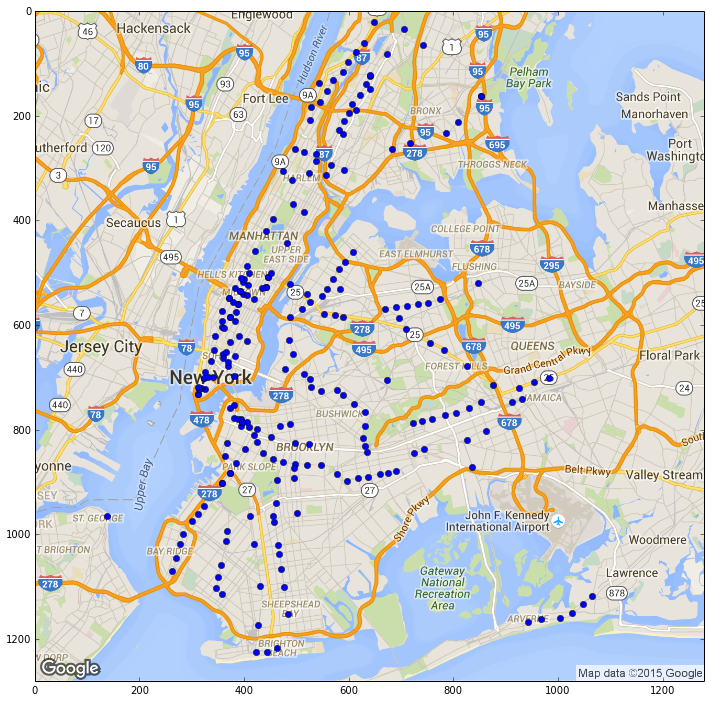
\includegraphics[scale=0.6]{map_stations.png}
\caption{Map of NYC subway stations}
\label{fig:subway_stations}
\end{figure}

\section{Meteorology}

\subsection{Meteorologic stations and their regions of responsibility}

The weather at the the subway UNITs is measured by meteo stations, located in the UNITs' vicinity. There are 37 meteorologic stations. A given meteo station can service one or more UNITs, and each UNIT is serviced by exactly one meteo station.

Although not required for this project, an effort was made to visualize also the location of the meteo stations. This was done together with calculating a theoretical \textbf{region of responsibility} for each station. The idea of this region is to determine which subway UNITs should be serviced by which meteo station. This calculation was done by performing a Voronoi tessellation of the mesh formed by the meteo stations. Figure \ref{fig:meteo_voronoi} shows these regions in a color-coded way, as per \cite{so_color_voronoi}. Additionally, it shows again the subway UNITs, this time color-coding them with the color of their servicing meteo station (as reported by the dataset). We see that most UNITs (not all!) have the same color as the Voronoi region in which they are located---this means that the Voronoi tessellation was a really good way to determine the extents of the area that is best served by a given meteo station. 

\begin{figure}[ht]
\centering
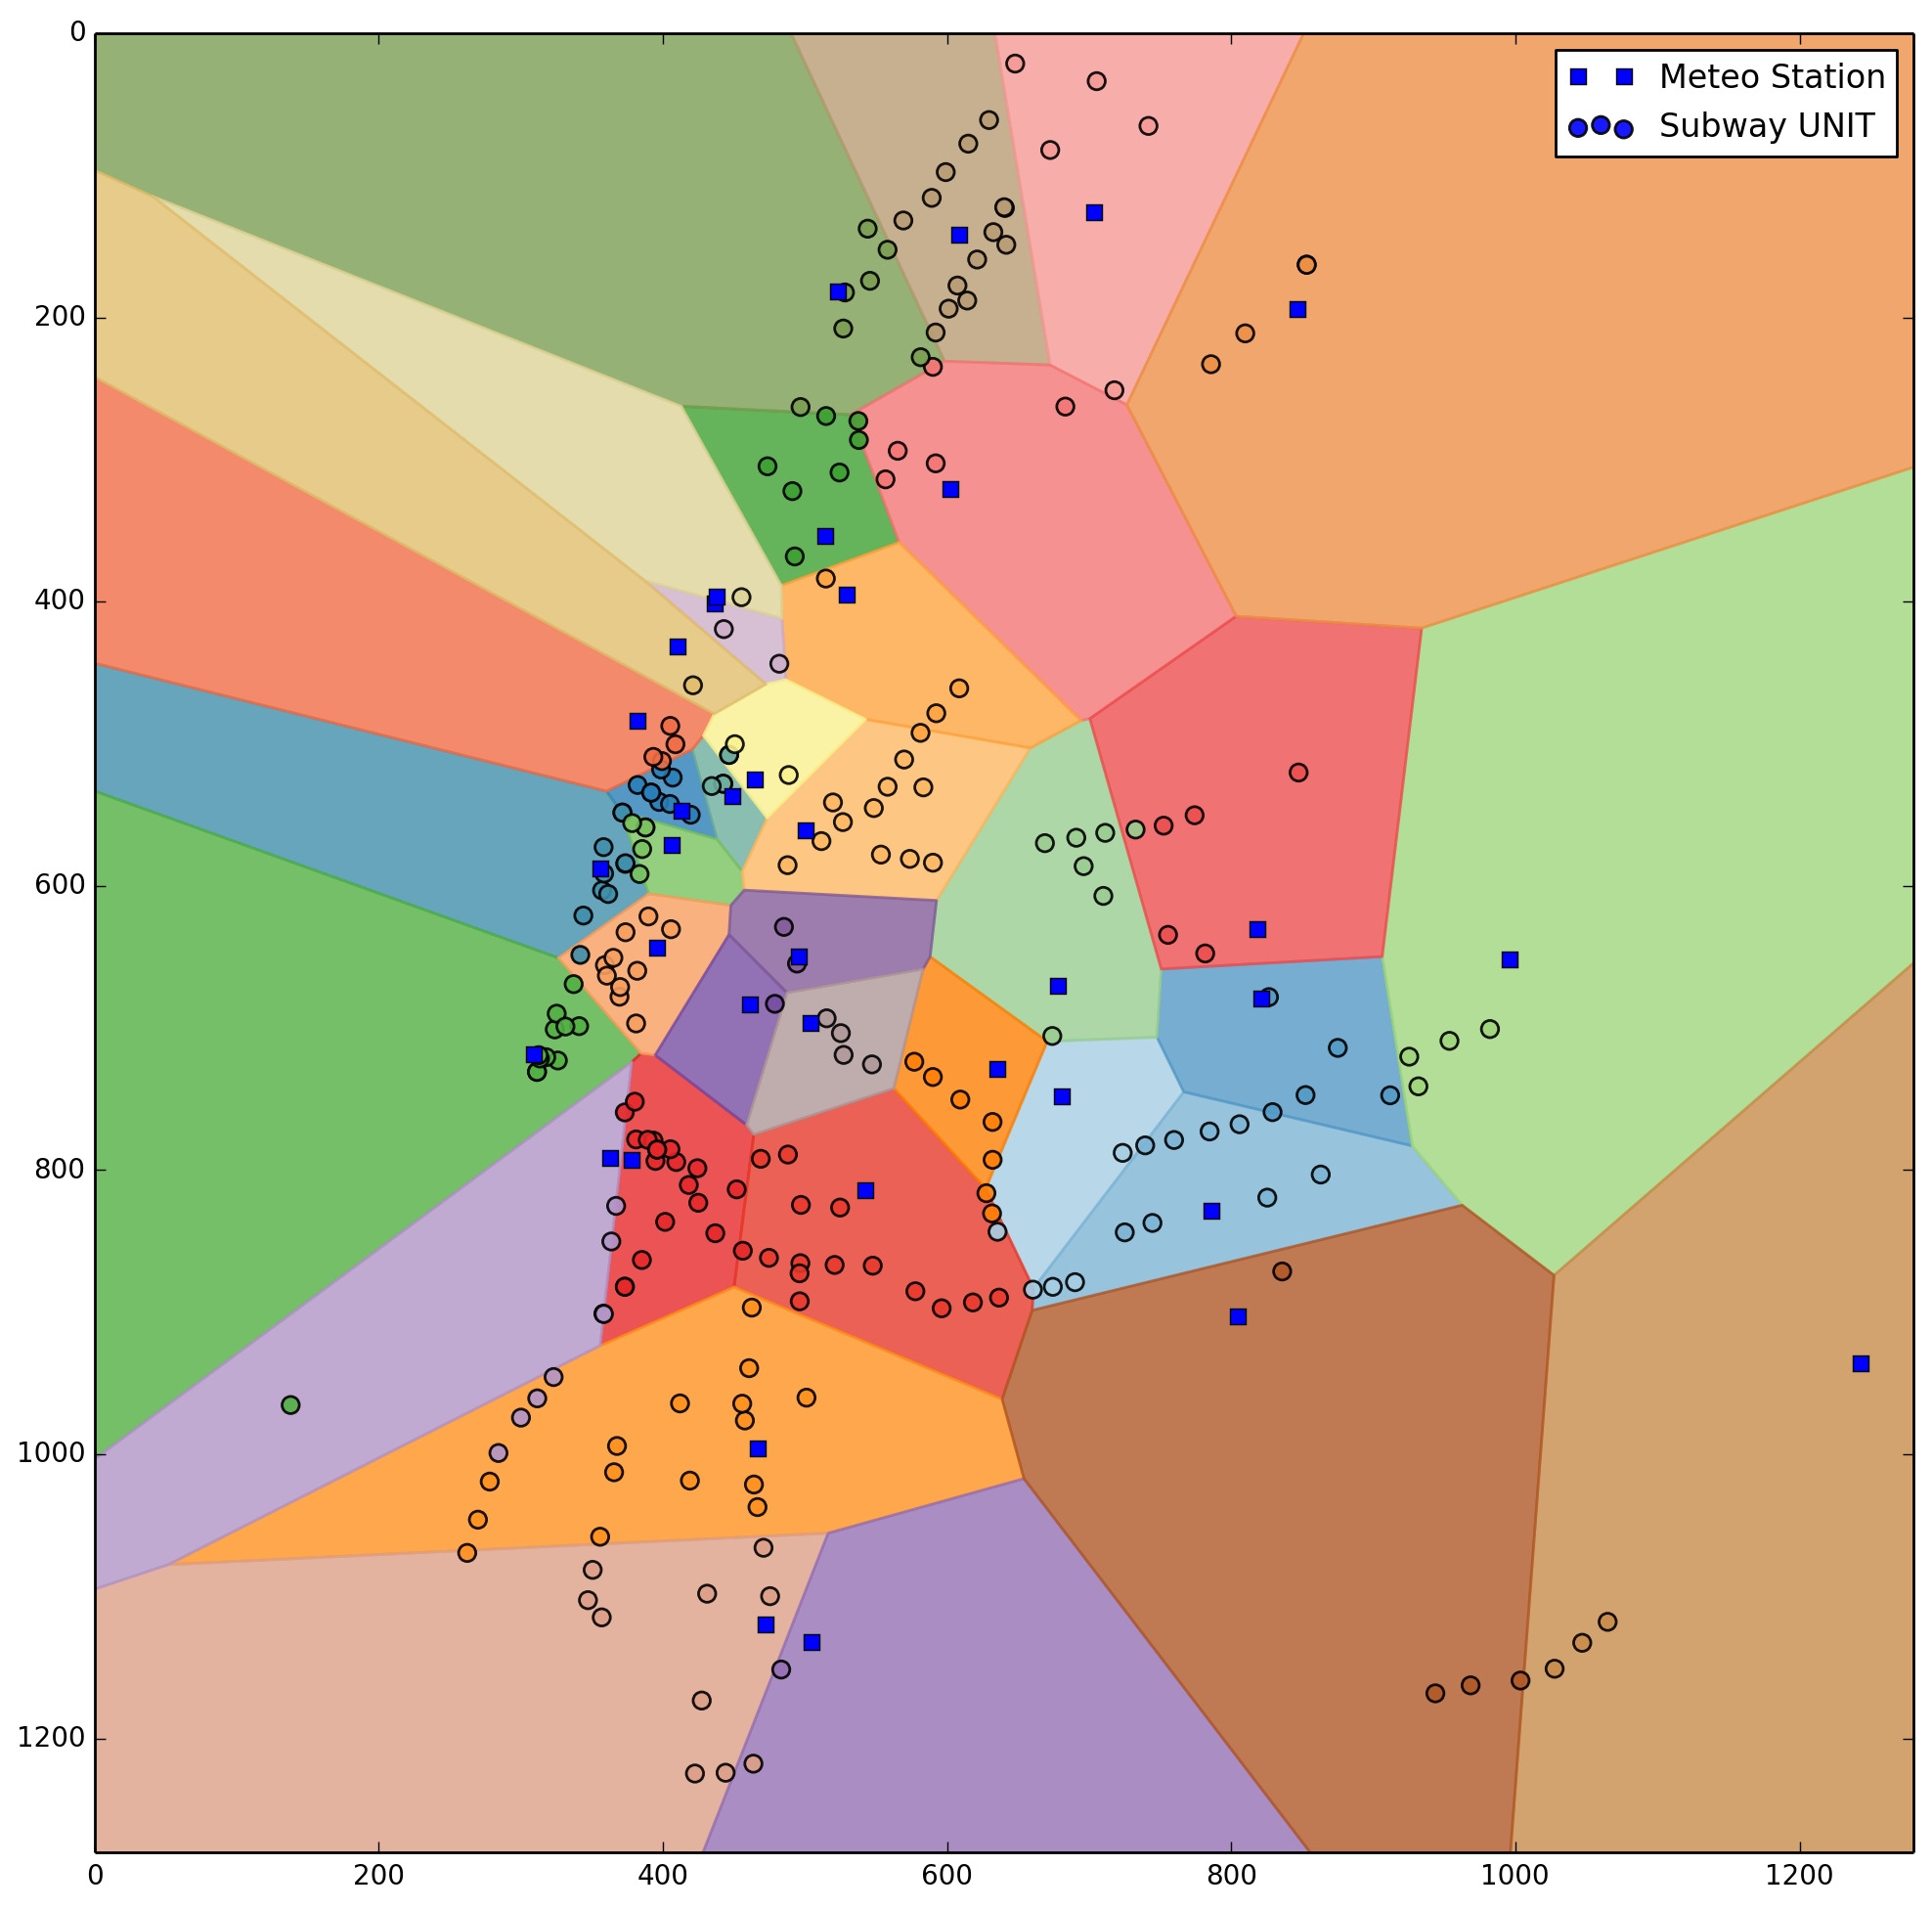
\includegraphics[scale=0.6]{meteo_voronoi.png}
\caption{Map of NYC meteo stations, their Voronoi-calculated regions of responsibility and subway UNITs}
\label{fig:meteo_voronoi}
\end{figure}

\subsection{Meteorologic conditions}

Using the Haversine geodesic formula (details in the IPython notebook), 
$$d = 2 r \arcsin \Bigg( \sqrt{ \sin^2 \bigg(\frac{\phi_2 - \phi_1} {2} \bigg) + \cos( \phi_2)\cos(\phi_1)\sin^2\bigg(\frac{\lambda_2 - \lambda_1} {2} \bigg) }\Bigg)$$
we find the \textbf{extents of the NYC subway area} to be approximately $35 \times 35 \ \rm km$. In this pretty big area we can expect to find different meteorologic conditions at different places at the same time.

Indeed, after performing some exploration with \tt pandas \rm of the initial dataset, we discover the following:
\begin{itemize}
\item It is possible for different subway stations to have different weather on the same day---so we cannot always talk about completely rainy or completely dry days for the whole subway.
\item Of the 31 days in the dataset, there are 9 days when we have had some subway stations receiving rain, while others not.
\item Of the remaining 22 days, during 21 of them the weather has been 100\% dry for all stations, while on 1 day (2011-05-17) we have had rain over 100\% of the subway.
\item Of the 9 "mixed weather" days, on '2011-05-19' we have had the most diversified rain conditions, i.e. almost half of the subway stations have been reporting rain, while the rest have been "dry". A map showing this can be seen in Figure \ref{fig:most-diverse-rain-conditions}.
\end{itemize}


\begin{figure}[ht]
\centering
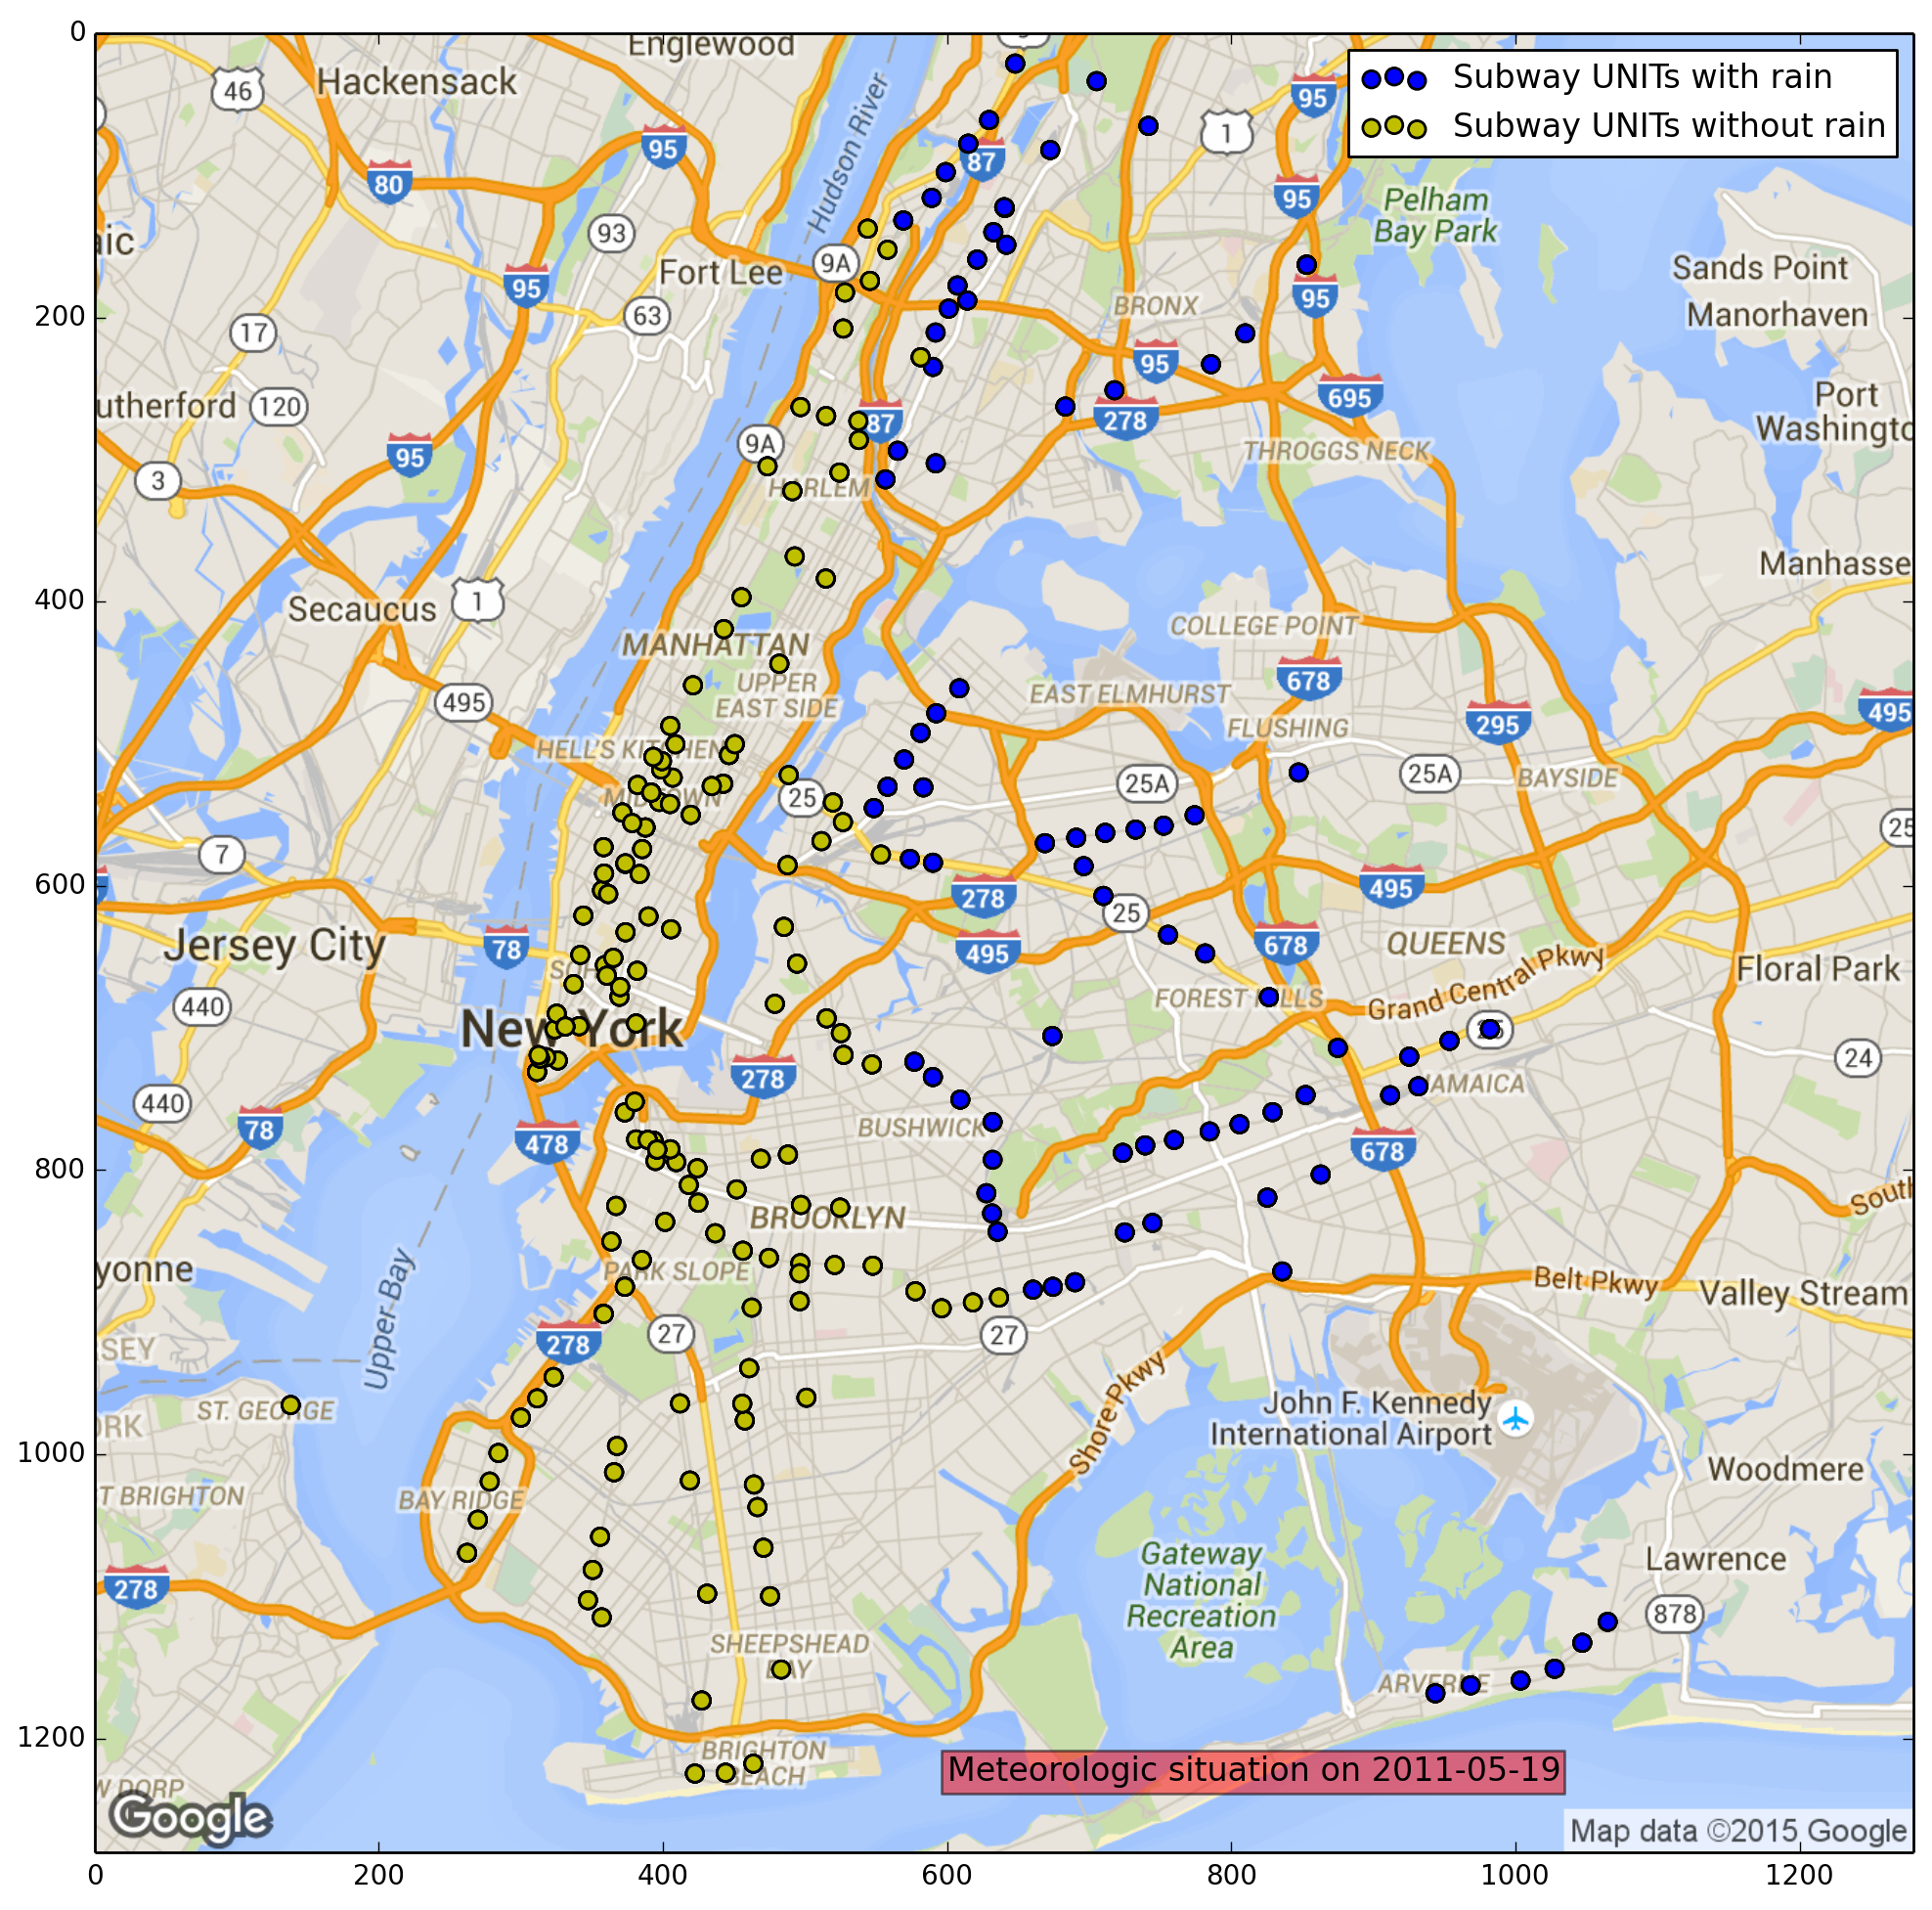
\includegraphics[scale=0.6]{map_half_rain_half_norain.png}
\caption{Map of NYC meteo stations, at the moment with most diversified rain conditions}
\label{fig:most-diverse-rain-conditions}
\end{figure}


\section{Predicting ridership}

\subsection{Brainstorming factors that can affect ridership}


Predicting the volume of ridership is not an easy task---there are simply too many known and unknown variables that can affect it. By intuition, we would expect the hourly number of entries into the subway to depend on factors like:

\begin{itemize}
\item \textbf{Time of the day}---Usually the morning hours will see more entries in stations located in residential regions; in the evening hours there should be more entries in  business areas stations.
\item \textbf{Day of the week}---Probably during the weekend there will be less subway entries.
\item \textbf{Location}---Stations located at transportation hubs, for example, probably will have more entries.
\item \textbf{Meteorologic conditions}---Do people prefer to take more the subway when it rains or is cold?
\item \textbf{State of the subway network}---Accidents, bottlenecks, jams or maintenance work somewhere on the subway network can reduce (or eliminate) the entries in some places and increase them in others.
\item \textbf{State of the other transportation networks (e.g. roads, buses and trains)}---All networks exhibit some kind of interdependence. Therefore problems on other networks (e.g. strikes of bus drivers, closed streets, etc.) can have profound effect on the subway usage.
\item \textbf{Significant public events}---Demonstrations, U.N. assemblies, big sport events, ticker-tape parades---all this can also significantly increase (or, on the contrary, block) the subway entries.
\end{itemize}

Figure \ref{fig:barplots_h_dw_wd_rain} shows barplots of the average entries as a function of some of the above factors; namely: time-of-day, day-of-week, weekend-or-weekday, and rain conditions. We see a really high dependence of the ridership on the time of the day and the day of the week, but much less pronounced dependence on the presence/absence of rain. We can draw the following conclusions:
\begin{itemize}
\item The weekends manifest significantly lower subway entries than the weekdays. This is an indication that the subway is heavily used for work commuting.
\item The highest number of subway entries are registered from the morning until after 20:00h---this corresponds to the period of highest economic and entertainment activity. 
\item Still, a little strange looks the relatively feeble entry activity at 8:00h, a time when we would expect a rush hour for the commuters. Probably this is due to the fact that NYC has the \textbf{latest median time} of arrival at work from all metro areas in the U.S., as reported in \cite{cities_sleep}.  
\end{itemize}

\begin{figure}[ht]
\centering
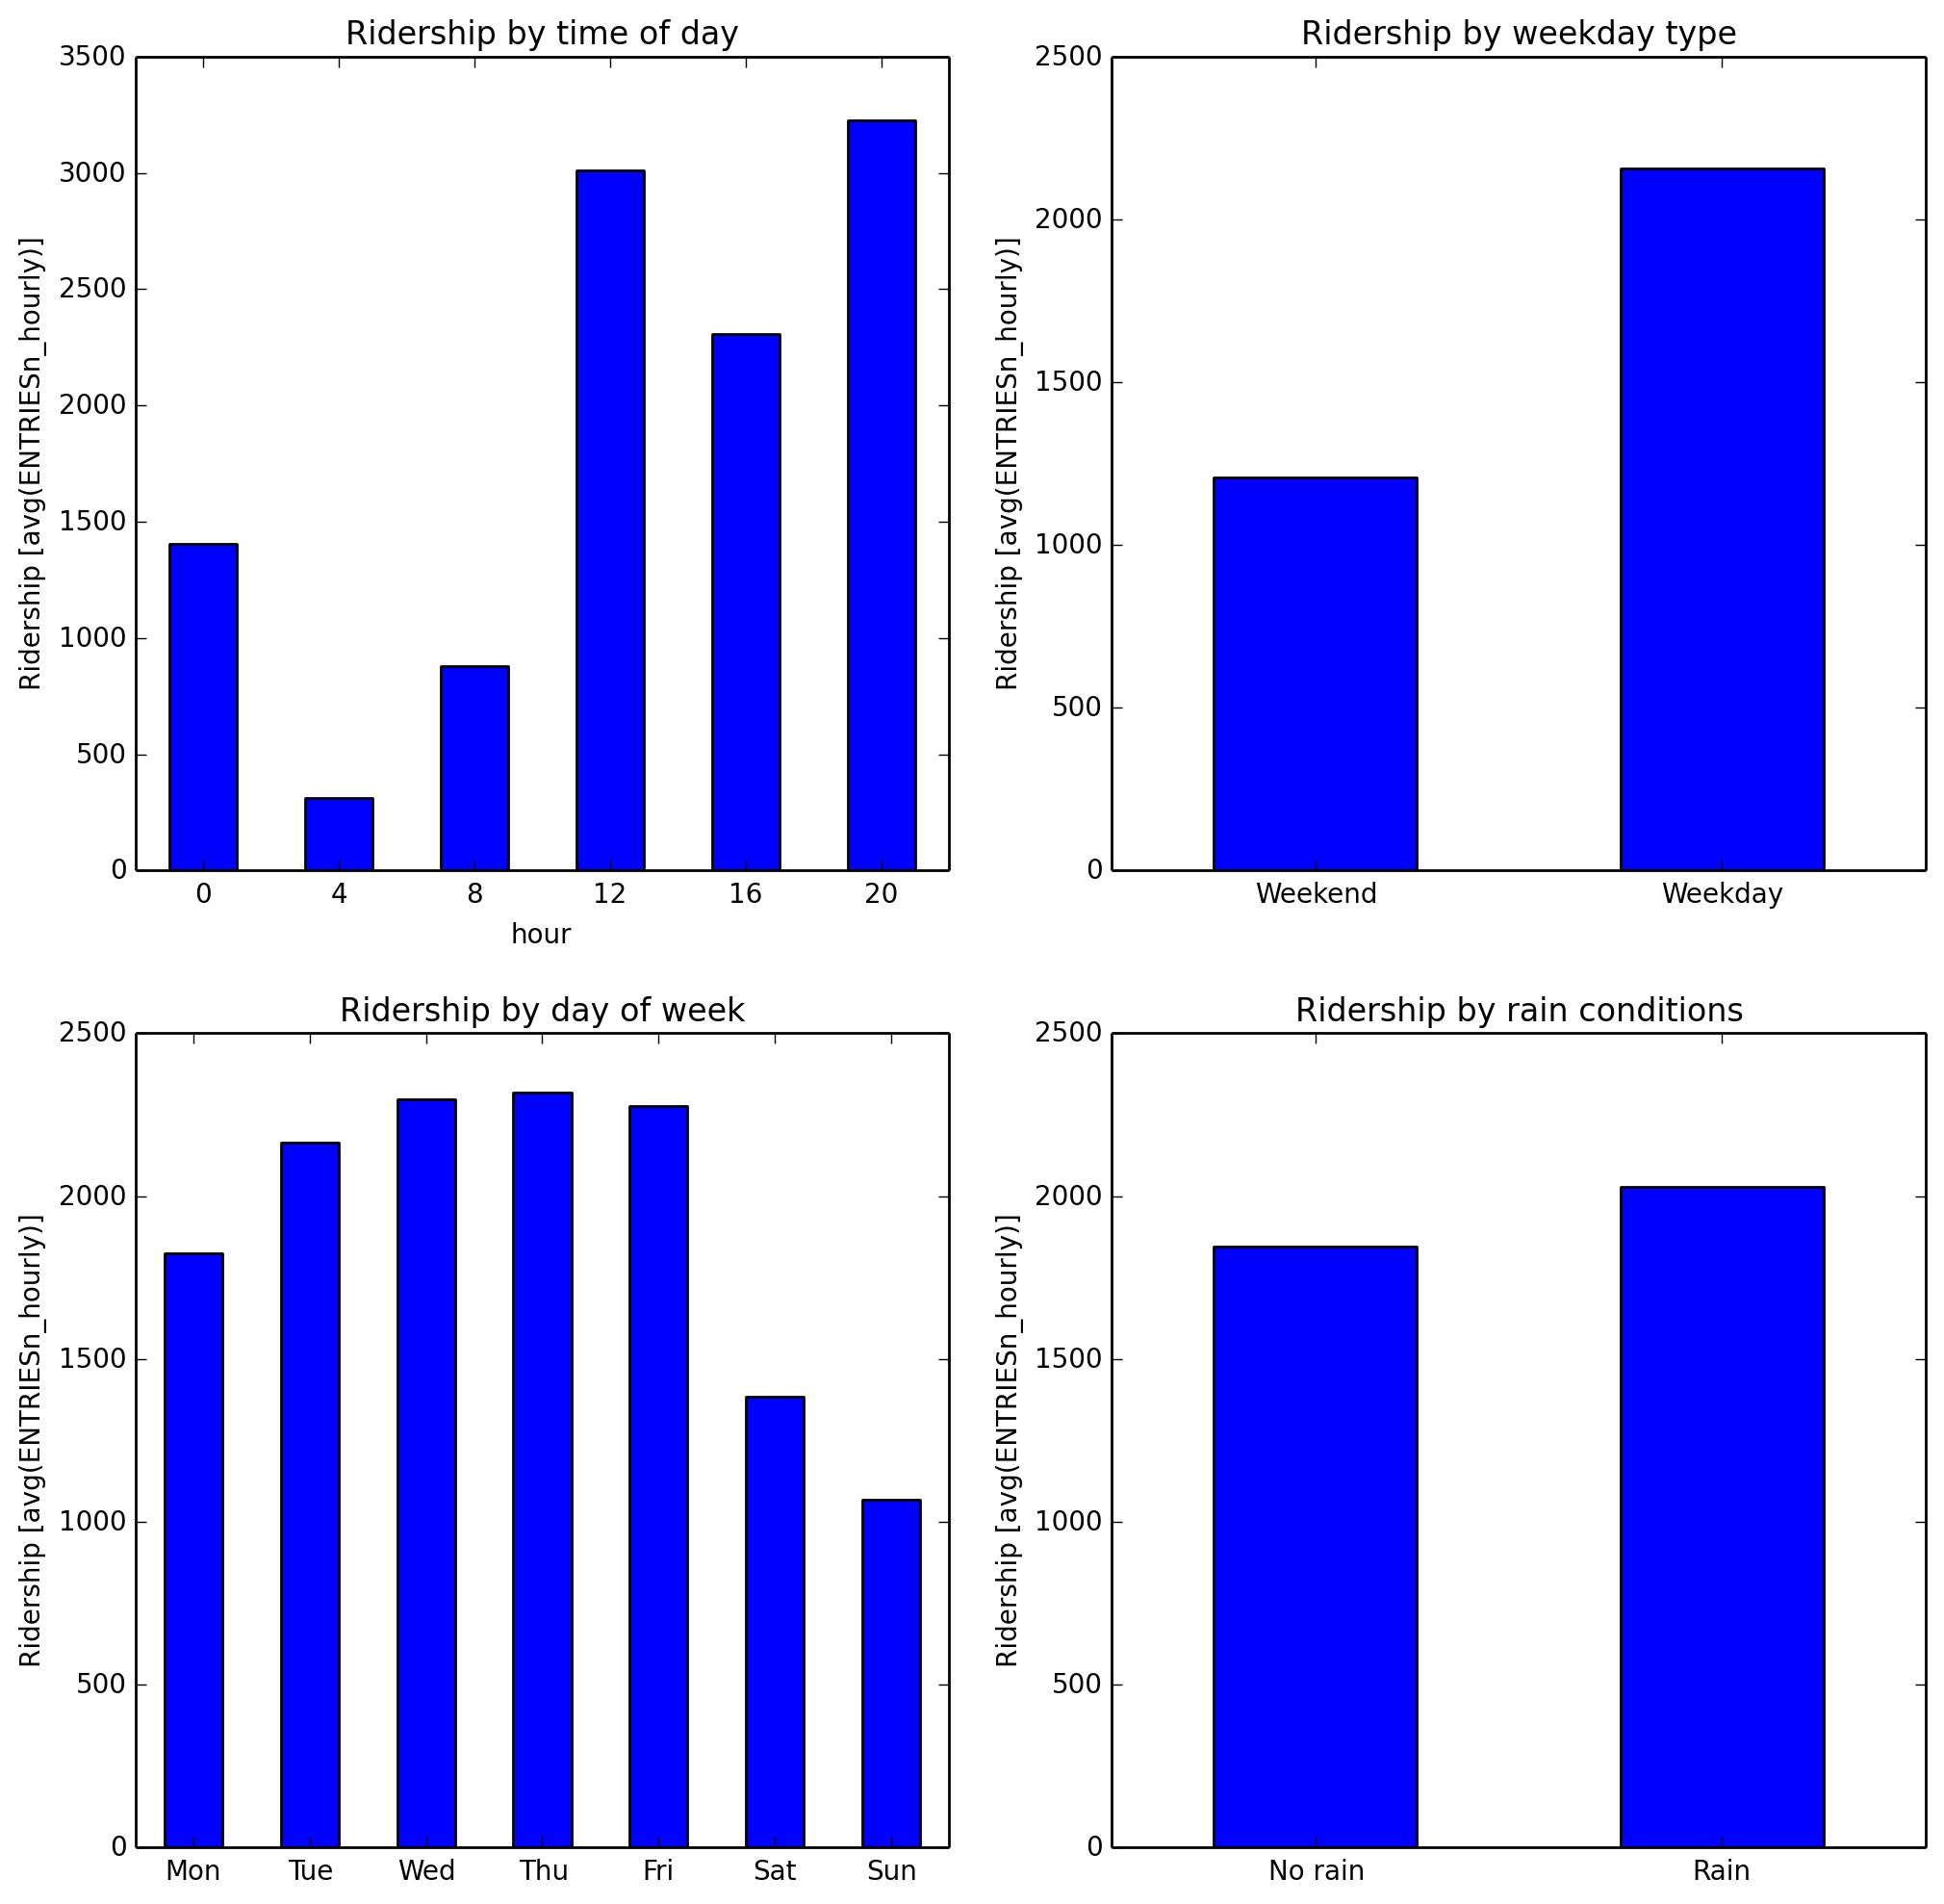
\includegraphics[scale=0.6]{barplots_ridership_hour_wkd_dow_rain.png}
\caption{Ridership as a function of several factors}
\label{fig:barplots_h_dw_wd_rain}
\end{figure}

To illustrate the ridership dependence on the location of the subway station, Figure \ref{fig:ridership-per-station} shows a map of the subway UNIT, where the size of the circles correspond to the average number of entries for the respective UNITs. We see especially numerous subway entries (bigger and more reddish circles)  in the following places:
\begin{itemize}
\item In Manhattan
\begin{itemize}
\item Grand Central Station, Times Square and 59-Columbus stations---important transportation hubs
\item Lower Manhattan---a distinguished business \& cultural center
 \end{itemize}
\item In Brooklyn
\begin{itemize}
\item Jamaica Center station---an important connection and hub for the passenger traffic from JFK airport.
\item Roosevelt Av. station---the same, but for La Guardia airport
 
\end{itemize}
\end{itemize}

\begin{figure}[ht]
\centering
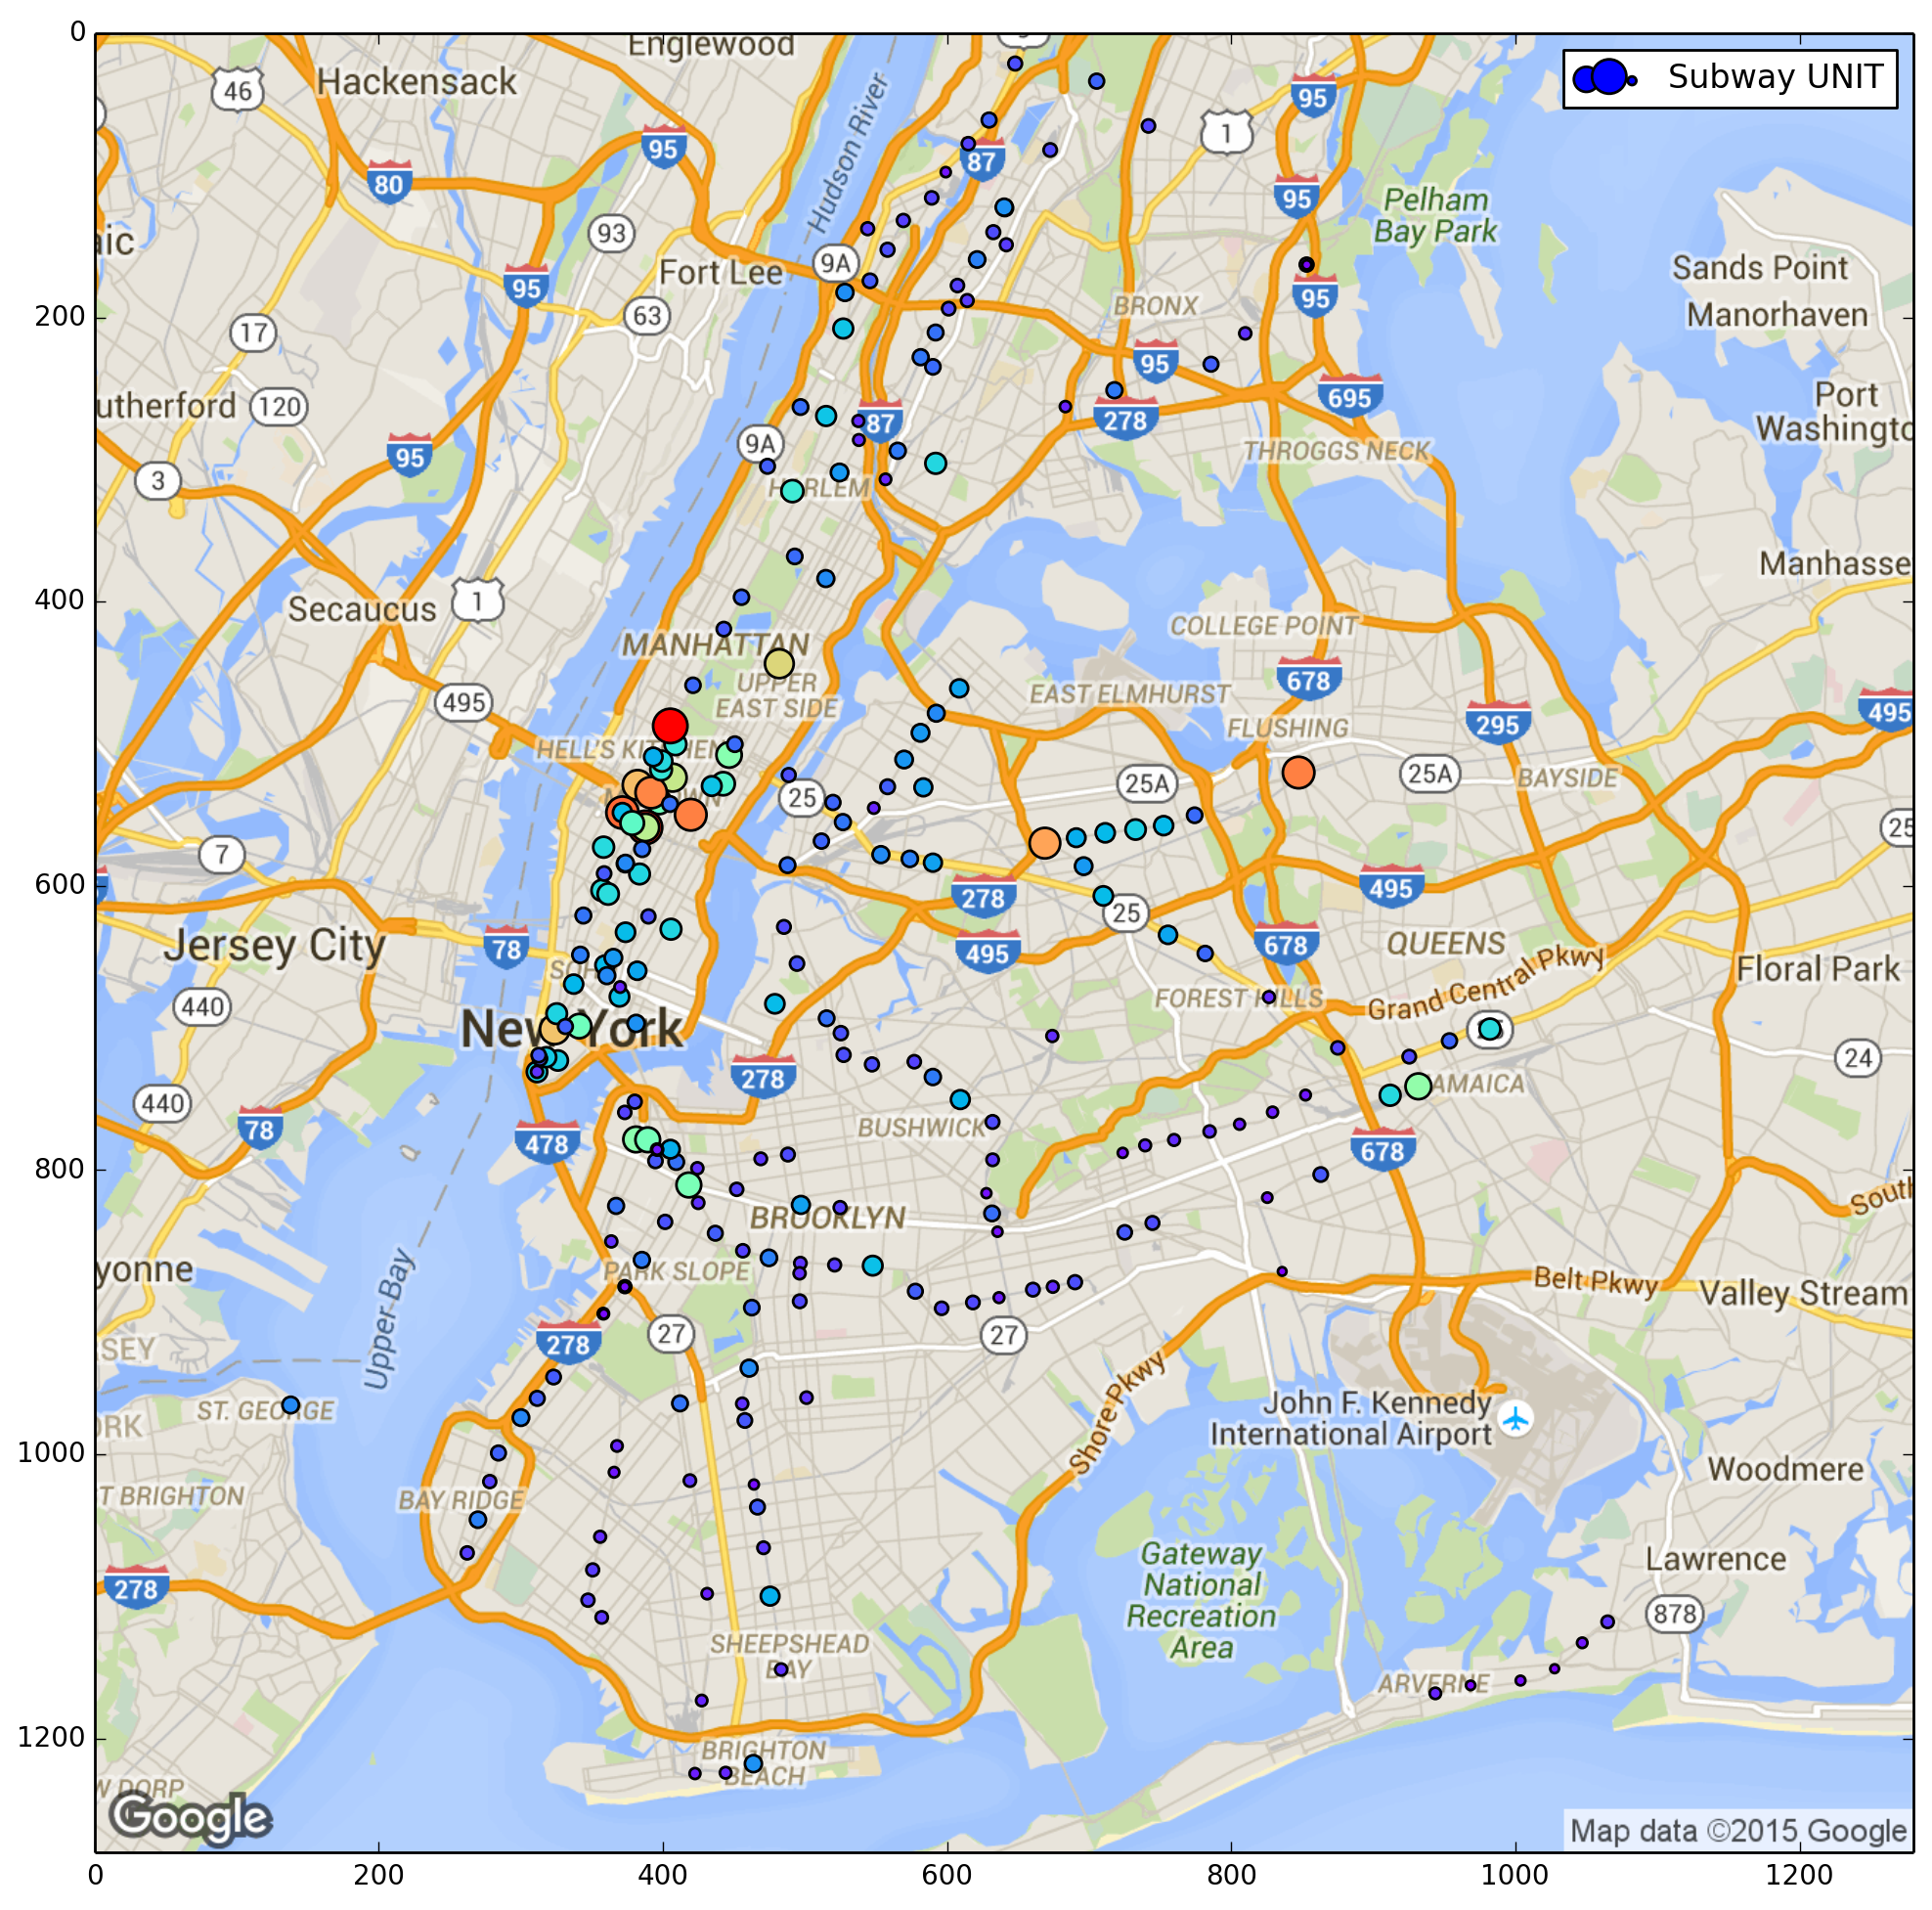
\includegraphics[scale=0.6]{map_stations_entry.png}
\caption{Ridership as a function of subway UNIT location}
\label{fig:ridership-per-station}
\end{figure}

In fact, table \ref{tab:top-ten-hourly} lists the top ten busiest stations according to our dataset. For comparison, the last column of the table shows the top-10 busiest stations according to the 2014 annual ranking given in \cite{mta_subway_data}.

\begin{table}[h!]
\centering
\begin{tabular}{c|l|c|c}
\hline
Rank & Station & Average hourly entries & Rank acc. to \cite{mta_subway_data} \\
\hline
1 & 59 ST-COLUMBUS  & 10046 & 7\\
2 & 42 ST-GRD CNTRL & 8360 & 2 \\
3 & MAIN ST         & 8359 & n/a \\
4 & 34 ST-HERALD SQ & 7851 & 3 \\
5 & ROOSEVELT AVE   & 7808 & n/a \\
6 & 42 ST-PA BUS TE & 7366 & n/a \\
7 & WORLD TRADE CTR & 7245 & n/a \\
8 & 47-50 ST-ROCK   & 6389 & n/a \\
9 & 42 ST-TIMES SQ  & 6363  & 1 \\
10 & JAMAICA CENTER  & 5364 & n/a \\
\hline
\end{tabular}
\caption{The top ten stations with highest hourly entries}
\label{tab:top-ten-hourly}
\end{table}

\subsection{Linear regression}

Next we will try to find a linear regression model for predicting the numbers of entries (ENTRIESn\_hourly) based on several exogenous variables. We can choose between \textit{Gradient Descent} and \textit{Ordinary Least Square (OLS)} methods for performing the linear regression. Gradient Descent is quicker but less precise (as it can get caught in local minima), while the OLS method is computationally more intensive, but also more precise (it is guaranteed to find the global minimum). Due to the small size of the input dataset, we \textbf{choose to use OLS}.

As we saw in the analysis above, the following variables have clear effect on the volume of ridership, therefore they make good candidates for becoming exogenous variables: hour, day\_week, UNIT (actually UNIT is the best proxy for the location of the subway station). We will be also interested in exploring the effect of the weather factors ('rain', 'fog', etc.) on the hourly entries.

The linear regression was performed with \tt statsmodel.api.OLS() \rm (see the accompanying IPython notebook) as shown in the following code:

\begin{lstlisting}[language=Python]
import statsmodels.api as sm

# Convert categorical variables to dummies
dummies_u = pd.get_dummies(df['UNIT'])
dummies_u.drop("R003", axis=1, inplace=True) # to avoid multicollinearity problems

# The exogenous variables
df_for_lr = df[["rain", "day_week", "hour"]]

# Add the intercept constant
df_for_lr["intercept"] = 1.0

# Add the dummies
df_for_lr = df_for_lr.join(dummies_u)

result = sm.OLS(df["ENTRIESn_hourly"], df_for_lr).fit()

print(result.summary())
\end{lstlisting}

Several experiments were performed, adding and removing exogenous variables and dummies, and recording the resulting \textbf{coefficient of determination $R^2$} to assess the prediction quality of the model. The results are summarized in table \ref{tab:lin_regr_exper}.


\begin{table}[ht]
\centering
\begin{tabular}{l|l|c|l}
\hline
Exogenous variables & Dummies & $R^2$ & Notes\\
\hline
day\_week, hour  & UNIT & 0.469 \\
day\_week, weekday, hour & UNIT & 0.483 & 'weekday' helps  \\
day\_week, weekday & UNIT, hour & 0.542 & Treating 'hour' as dummy helps \\
day\_week, weekday, rain & UNIT, hour & 0.542 & 'rain' doesn't help \\
day\_week, weekday, rain, precipi & UNIT, hour & 0.542 & 'precipi' doesn't help \\
day\_week, weekday, rain & UNIT, hour, conds & 0.543 & 'conds doesn't help \\
day\_week, weekday, rain, tempi & UNIT, hour & 0.543 & 'tempi' doesn't help \\
day\_week, weekday, meanprecipi & UNIT, hour & 0.542 & 'meanprecipi' doesn't help \\
day\_week, weekday, meantempi & UNIT, hour & 0.542 & 'meantempi' doesn't help \\
day\_week, weekday, fog & UNIT, hour & 0.542 & 'fog' doesn't help \\
day\_week, weekday, pressurei & UNIT, hour & 0.542 & 'pressurei' doesn't help \\
\hline
\end{tabular}
\caption{Experimenting with different exogenous variables for the OLS Linear Regression}
\label{tab:lin_regr_exper}
\end{table}

We clearly see that the only variables that contribute to the predictive power of the model are: \textbf{day\_week, weekday, hour, UNIT}. The weather-related factors, on the other hand, had no significant influence on the precision.

Table \ref{tab:ols_results} shows the non-dummy coefficient weights from one of the OLS experiments.

\begin{table}[ht]
\centering
\begin{tabular}{l|c|c|c}
\hline
Factor & Weight $\theta$ & \multicolumn{2}{|c}{[95\% CI]}\\
\hline
intercept &  -1421.89 & -1741.07 & -1102.71\\
day\_week &  72.22 &   56.75 & 87.69 \\
weekday &  1272.51 &  1200.94 &  1344.09 \\
rain  & 32.19 & -13.85 &  78.22\\
\hline
\end{tabular}
\caption{Resulting weights from one of the OLS Linear Regression experiments}
\label{tab:ols_results}
\end{table}

We notice that the 95\% CI for the 'rain' factor is pretty wide. This indicates a rather uncertain, non-robust factor; a fact corroborating our finding that it adds virtually nothing to the predictive power of the model. In comparison, the other factors have narrower CIs, and as a consequence clearer effect on the predictions.

We can plot the residuals after applying the above model by:
\begin{lstlisting}[language=Python]
(df.ENTRIESn_hourly - result.fittedvalues).hist(bins=40)
\end{lstlisting}

The residues histogram is show in figure \ref{fig:residues}. We see that around 20\% of the residues have significant amplitude reaching 50\% of the range of the dependent value. At the same time the residues are not very well behaved (see \cite{good_residues}), since they exhibit a positive skew---probably suggesting the existence of undiscovered higher-order factors.

This (as well the relatively low value of $R^2=0.542$) is an indication that the Linear Regression is \textbf{not an adequate data prediction model} for this dataset. Other methods for machine learning, like \textit{Random Forests} could be more appropriate.

\begin{figure}[ht]
\centering
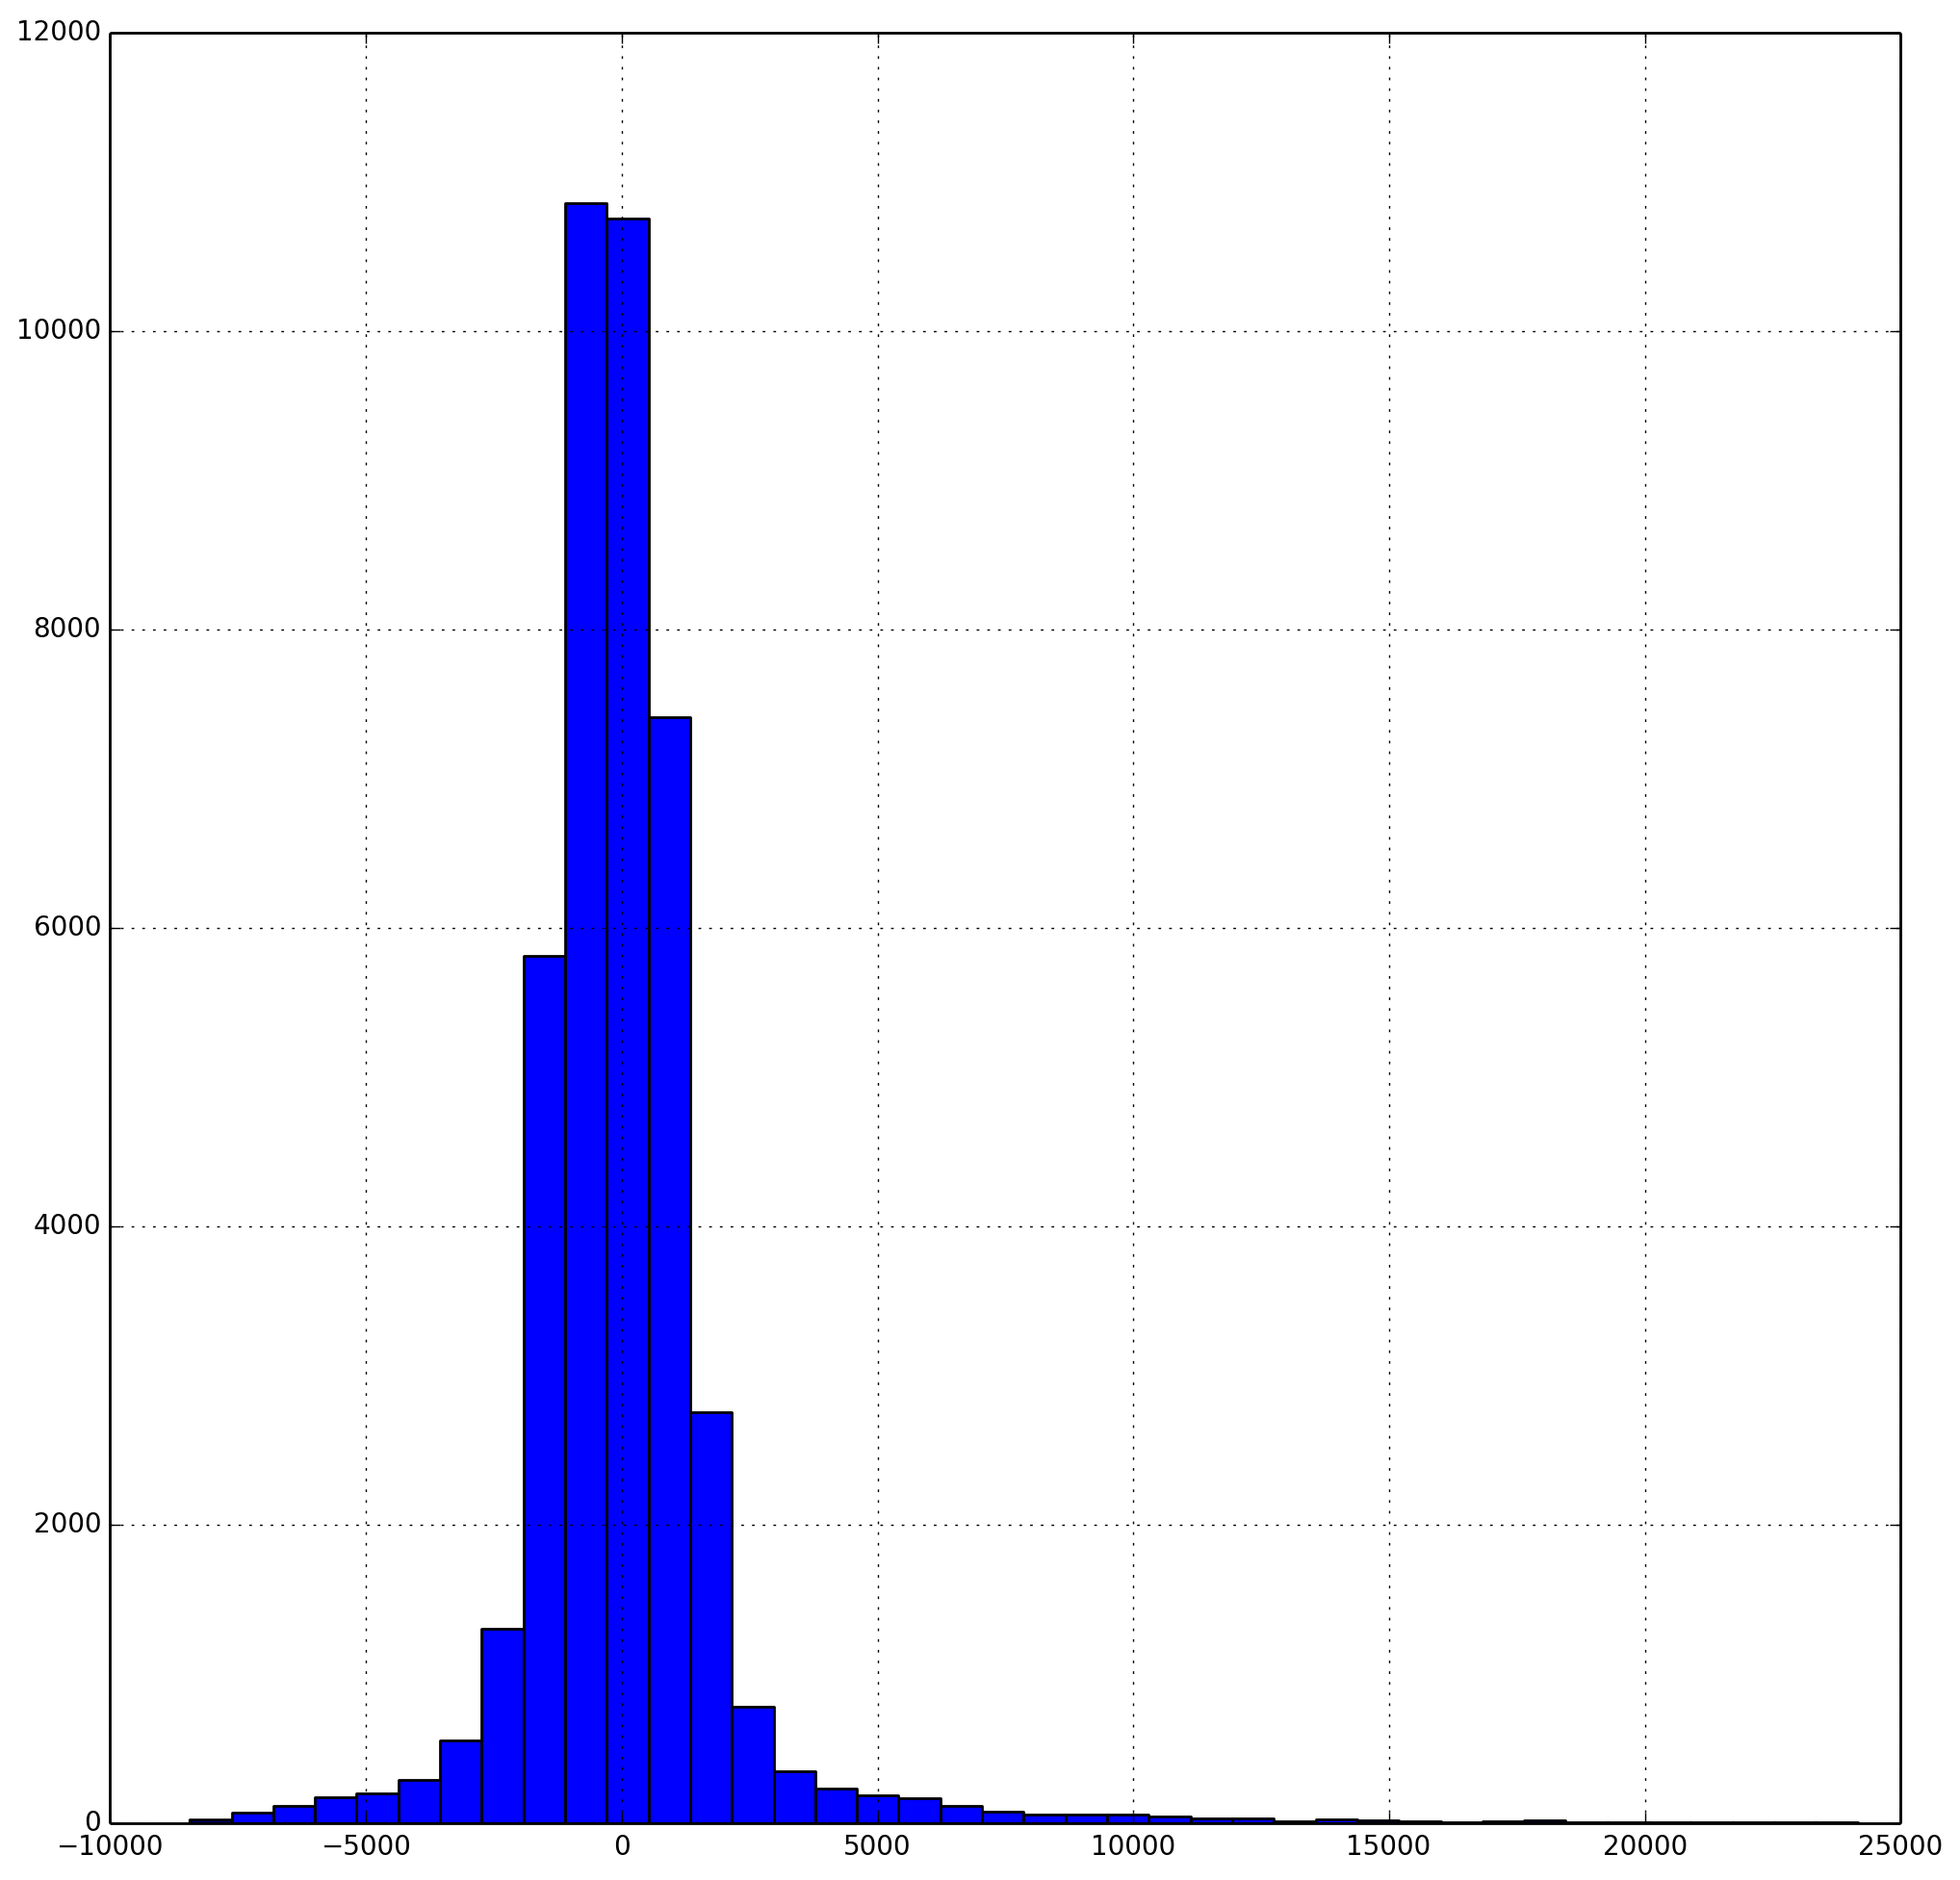
\includegraphics[scale=0.6]{residues.png}
\caption{Histogram of residues after applying the OLS model on the initial dataset}
\label{fig:residues}
\end{figure}

\section{Statistical test of ridership on rainy and dry days}

\subsection{Selecting an appropriate statistical test}
Before selecting an appropriate statistical test we have to explore the distribution of the data. Figure \ref{fig:histo_rainy_dry} shows the two superimposed hourly entries' histograms for rainy and dry days. We see that the two samples have \textbf{identical} distributions, which however are \textbf{not normal}. Therefore we cannot use tests like Welch's T-test, that require normal distribution of the observations. We shall instead use a non-parametric test, like the rank-sum based \textbf{Mann-Whitney U test.}

\begin{figure}[ht]
\centering
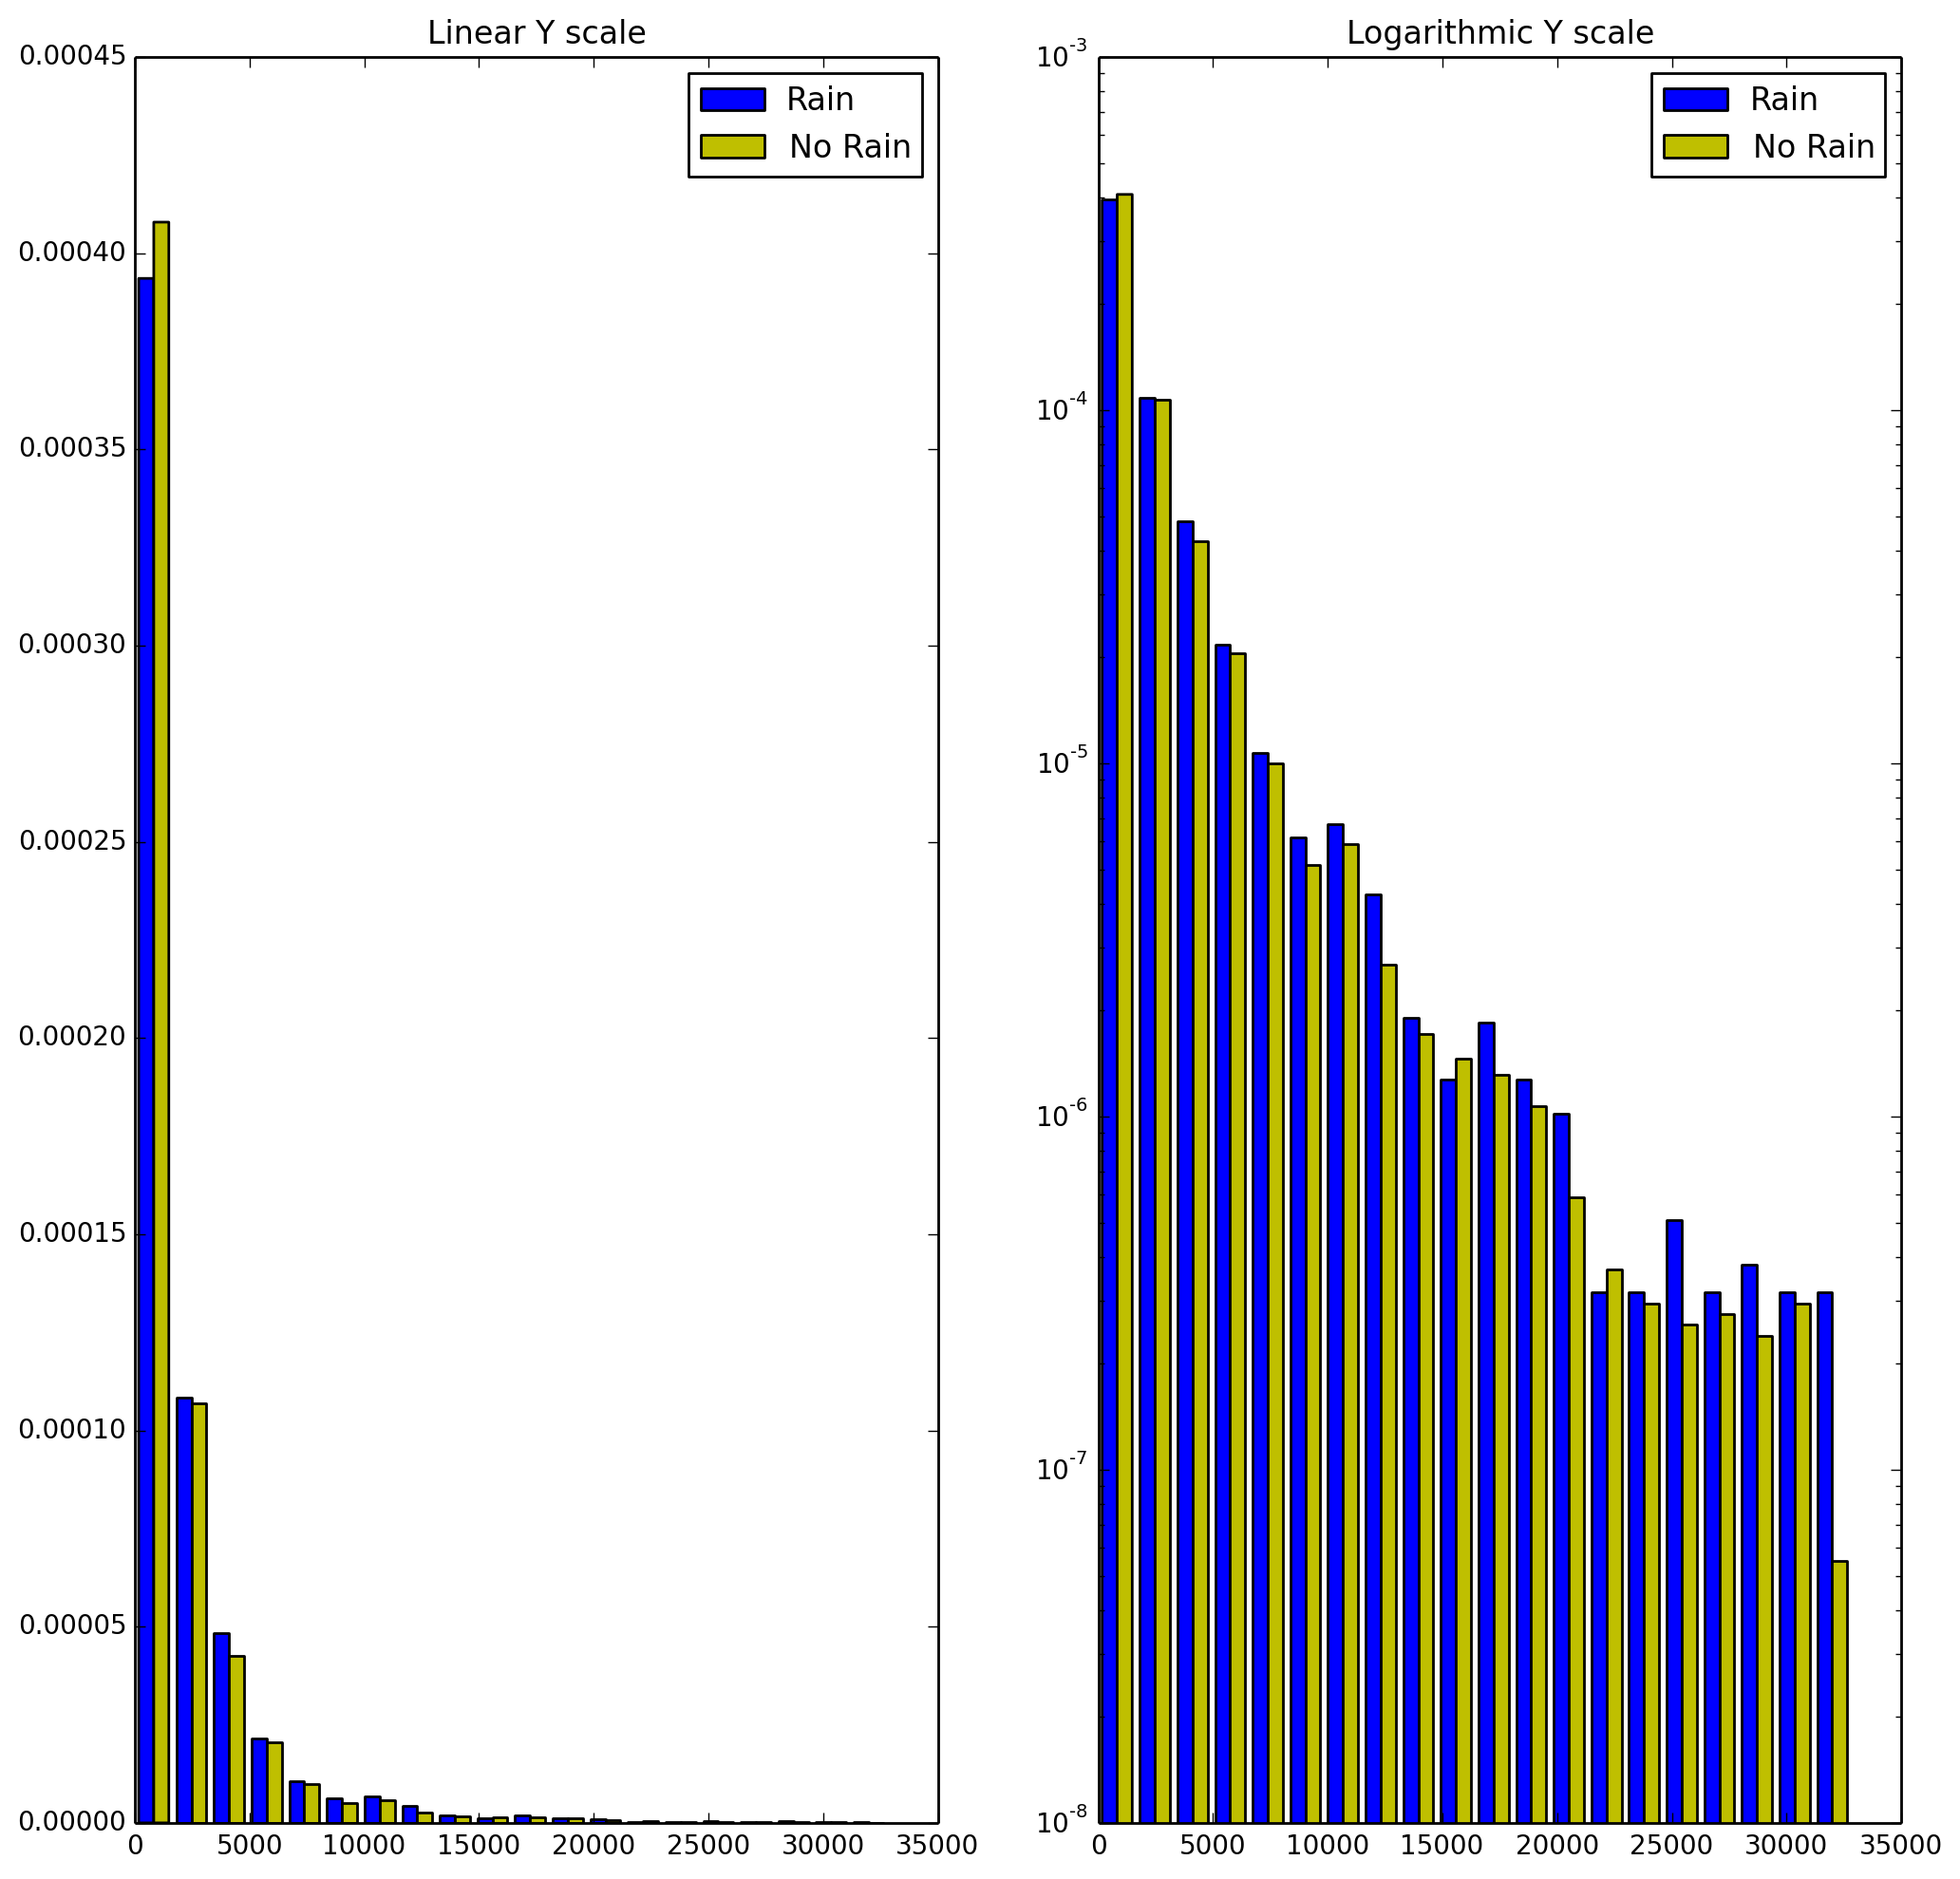
\includegraphics[scale=0.6]{histo_rainy_dry.png}
\caption{Histogram of ridership on rainy and dry days}
\label{fig:histo_rainy_dry}
\end{figure}

\subsection{Applying the Mann-Whitney U test}

\subsubsection{Assumptions}
According to \cite{mannwhitney_spss}, the input dataset need to fulfill the following requirements in order to be acceptable for a Mann-Whitney U test:
\begin{itemize}
\item Have one \textbf{dependent continuous or ordinal} variable---this is fulfilled as our dependent variable is the hourly count of entries into the subway.
\item Have one \textbf{independent categorical dichotomous} variable, consisting of two independent groups---this is fulfilled as our independent variable has two independent levels: "rain" and "no rain".
\item Have \textbf{independence of observations}, i.e. there shall be no relationship between the observations in each group of the independent variable or between the groups themselves. To ensure this we must have different participants in each group with no participant being in more than one group. This requirement in fact is something that needs to be guaranteed by the test design, and is not something that can be tested for. In our case this is also fulfilled, since each observation represents an \textbf{unique combination of \tt UNIT \rm and \tt datetime \rm}. If this assumptions were not fulfilled, we could have used the \textbf{Wilcoxon signed-rank test} instead.
\end{itemize}

\subsubsection{Hypothesis}
Furthermore, if the distributions of the two samples have the \textbf{same shape}, we can use the Mann-Whitney U test to compare the much more intuitive \textbf{median} statistics of the samples, rather than their \textbf{mean ranks}.

In our case, we have same-shaped distributions, therefore we can postulate the following hypotheses:
\begin{itemize}
\item \textbf{Null-Hypothesis, $H_0$}: the distributions of the two groups are equal (identical)
\item \textbf{Alternative Hypothesis, $H_a$}: the median of the two sample groups are statistically different.
\end{itemize}

This formulation of the hypotheses calls for a \textbf{two-tailed} statistical test.

\subsubsection{Mann-Whitney U test results and their representation}

The statistical test was performed via \tt scipy.stats.mannwhitneyu() \rm (see the accompanying IPython notebook):

\begin{lstlisting}[language=Python]
U, p = scipy.stats.mannwhitneyu(df[df.rain==0].ENTRIESn_hourly, 
                                df[df.rain==1].ENTRIESn_hourly)
\end{lstlisting}

The returned result was: $$ U = 153635120.5, \ \ p=2.74x10^{-6}$$

Since the scipy implementation of the test returns a one-tailed p-value, we have to multiply it by 2 to obtain the two-tailed value:
$$ p=5.48x10^{-6} \ \rm (two-tailed)$$

Since the critical p-value ($\alpha-level$) is conventionally set at 0.05, we have enough statistical evidence ($p<<p_{crit}$) to \textbf{reject the null-hypothesis}, i.e. we prove a significant difference between the two samples. 

The median values of hourly entries between the rainy and dry observations calculated via:

\begin{lstlisting}[language=Python]
df[df.rain==0].ENTRIESn_hourly.median()
df[df.rain==1].ENTRIESn_hourly.median()
\end{lstlisting}

are pretty close: 
$$\widetilde{entries}_{rain} = 939 \ \ \ \widetilde{entries}_{dry} = 893$$

This also gives an effect size (samples median difference) of $939-893=46$ in favor of the rainy days.

Following \cite{wiki_mwu} we can report our findings as follows:

\textit{Median number of hourly subway entries for groups "rain" and "no rain" are 939 and 893 respectively; the two group distributions were found to be statistically different (Mann–Whitney $U = 153635120.5,\ n_{rain} = 9585,\ n_{dry} = 33064,\ P < 0.05\ \rm two-tailed)$. We can therefore conclude that the analyzed dataset indicates a significant difference between subway entries on rainy and non-rainy days, with an effect size of 46.}


\section{Conclusion}

The performed non-parametric Mann-Whitney U test did indicate a significant difference between the volumes of ridership on rainy and non-rainy days; so, people really ride more the subway on rainy days.

At the same time we saw that 'rain' is not a significant predictor in a Linear Regression model trained on the given dataset, i.e. it does not help us predict reliably ridership.

\section{Reflection}

There are some shortcomings related to the input dataset:
\begin{itemize}
\item The records span only a very short period of time---one calendar month---thus we cannot estimate any effects related to the seasonal changes.
\item To improve the quality of the prediction models, collecting data about additional factors could be useful: e.g. maintenance work on the subway, closed down lines, black-outs, presence of big public events, disturbances on alternative transportation networks (e.g. blocked roads).
\end{itemize}

\medskip

\printbibliography

\end{document}
